\subsection{Postprocessing}
\subsubsection[Linearer Layout Optimierer]{Linearer Layout Optimierer \myAuthor{Sami Hamza}}
\paragraph{Motivation} Ziel des Linearen Layout Optimierers ist es die Puzzleteile anhand ihrer detektierten Ecken möglichst gut anzuordnen. Im Gegensatz zu einem greedy Ansatz soll hier jedoch ein globales Optimum gefunden werden. Hierfür wird vorausgesetzt, dass die Korrespondenzen der jeweiligen Puzzleteilkanten bereits bekannt sind. 
\paragraph{Herleitung des Least Square Problem}
Gegeben ist ein gelöstes Puzzle $P$ mit $N$ Zeilen und $M$ Spalten, wobei jedes Puzzleteil $P_i$ eine lokale Basis ${}^{(i)}B$ erhält. Die Basen der Puzzlteile ${}^{(i)}B$ befinden sich im jeweiligen Bildzentrum und weisen parallele Achsen zum Bildkoordinatensystem auf (siehe. \autoref{fig:base}). Somit können die im Bildkoordinatensystem ${}^{(i)B_{img}}$ angegebenen Koordinaten der Exkpunkte durch einfaches subtrahieren den Offset-Vektors (von ${}^{(i)}B_{img}$ zu ${}^{(i)}B$) ermittelt werden. Im Folgenden werden alle Größen stets im zentrierten Koordinatensystem betrachtet. Als Skaleneinheit wird stets die Einheit Pixel verwendet.

\begin{figure}[H]
    \begin{minipage}[t]{0.45\textwidth}
        \centering
        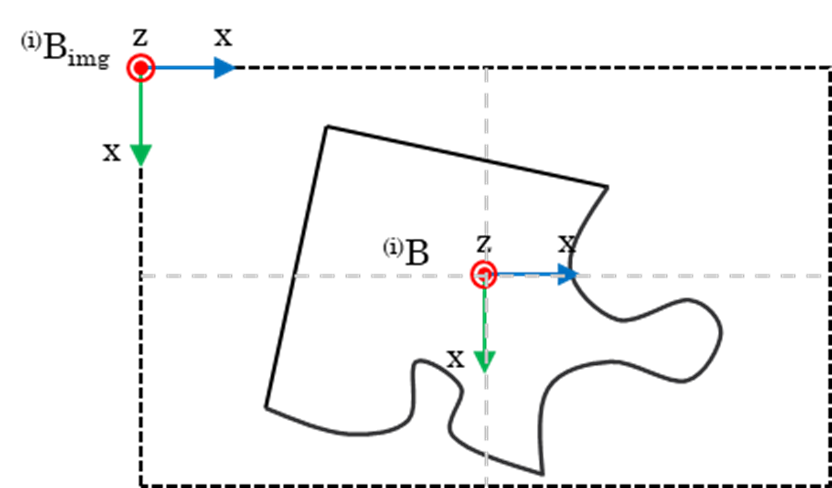
\includegraphics[width=0.95\textwidth]{sections/solver/images/base.png}
        \caption{Platzierung des Puzzleteilbasen.}
        \label{fig:base}
        \end{minipage}
    \hfill
    \begin{minipage}[t]{0.45\textwidth}
        \centering
        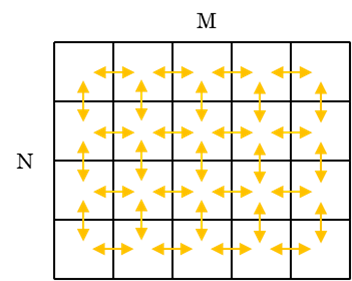
\includegraphics[width=0.7\textwidth]{sections/solver/images/puzzle_grid_and_corr.png}
        \caption{Puzzle-Gitter mit Korrespondierenden Kanten (durch gelbe Pfeile markiert).}
        \label{fig:puzzle_grid}
    \end{minipage}
\end{figure}

Zu Beginn muss eine Fehlermetrik aufgestellt werden, über welche die Qualität der Optimierung ermittelt werden kann. Hier werden die Vektoren $\epsilon_{(i,n),(j,k)}$ zwischen korrespondierenden Ecken $n$ und $j$ zweier benachbarter Kanten der Teile $i$ und $j$ im Referenzsystem ${}^{(0)}B$ gewählt (vgl. \autoref{fig:error_metric}).

\begin{figure}[H]
    \centering
    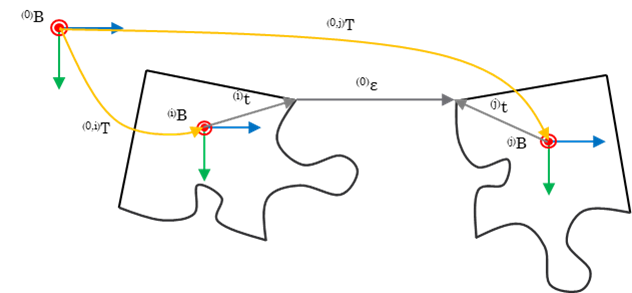
\includegraphics{sections/solver/images/error_metric.png}
    \caption{Veranschaulichung der Ermittelung der Fehlermetrik.}
    \label{fig:error_metric}
\end{figure}

Daraus resultieren zwei Vektoren pro Kantenpaar. Idealerweise betragen alle Vektoren einen Wert von Null. Die Fehlervektoren $\epsilon_{(i,n),(j,k)}$ können anschließend wie folgt im globalen System beschrieben werden
\begin{equation}
    \epsilon_{(i,n),(j,k)} = {}^{(0,i)}T  {}^{(i)}t_n - {}^{(0,j)}T {}^{(j)}t_k
\end{equation}
Dabei geben ${}^{(i)}t_n$ bzw. ${}^{(j)}t_k$ jeweils die Koordinaten der korrespondierenden Eckpunkte in ${}^{(i)}B$ bzw. ${}^{(j)}B$ an. Außerdem entspricht ${}^{(0,i)}T \in SE2$ der Pose der Basis ${}^{(i)}B$ im Referenzsystem, welche durch eine homogene Matrix im $\mathbb{R}^2$ ausgedrückt werden kann. Diese beinhaltet eine druch den Rotatinoswinkel $\phi_{r,i}$ parametrisierte Rotationsmatrix $R_z(\phi_{r,i}) \in SO2$, die eine Rotation um die z-Achse beschreibt und sich aus einem Vorrotationswinkel $\
\phi_{0,i}$ (aus der groben Lösung des Puzzles) und einem Feinjustierwinkel $\phi_{i}$ zusammensetzt, und eine durch $x_i$ und $y_i$ parametrisierte Translation $r(x_i,y_i) \in \mathbb{R}^2$ des Ursprungs.
\begin{gather}
    {}^{(0,i)}T = 
    \begin{bmatrix}
        R_z(\phi_{r,i}) & r(x_i,y_i)\\
        \mathbf{0} & 1
    \end{bmatrix} \text{, mit }\\
    R = 
    \begin{bmatrix}
        cos(\phi_{0,i} + \phi_{i}) & -sin(\phi_{0,i} + \phi_{i})\\
        sin(\phi_{0,i} + \phi_{i}) & cos(\phi_{0,i} + \phi_{i})
    \end{bmatrix} \text{ und } \label{gl:rotmat}
    r = 
    \begin{bmatrix}
        x_i\\
        y_i
    \end{bmatrix}
\end{gather}

Das Ziel der Optimierung ist also die Minimierung des Least Squares Problems aus Summe der euklidischen Norm der Fehlervektoren der Menge aller Korrespondierender Ecken $K$ (hier keine Betrachtung von doppelten Korrespondenzen (i,j) und (j,i) und keine Betrachtung diagonaler Teilkorrespondenzen).
\begin{equation}
    \arg\min_x \frac{1}{2} \sum^{|K|} \lVert \epsilon(x) \rVert_2^2 \label{gl:leastsquare}
\end{equation}
Der Parametervektor $x$ setzt sich zusammen aus den Parametrisierungen für die Posen der Puzzleteile und beinhaltet somit pro Puzzleteil drei Parameter $x \in \mathbb{R}^{3|P|}$.
\begin{equation}
    x = \begin{bmatrix}
        \phi_i & x_i & y_i & \dots & \phi_{|P|} & x_{|P|} & y_{|P|}
    \end{bmatrix}^T
\end{equation}

Es wäre für eine effiziente Optimierung von Vorteil, wenn die ein linearer Zusammenhang $\epsilon = Ax+b$ zwischen den Fehlervektoren $\epsilon$ und dem Parametervektor $x$ besteht. Dieser kann durch heranziehen der Kleinwinkelnäherung und Additionstheoremen für die in \autoref{gl:rotmat} definierte Rotationsmatix hergestellt werden.
\begin{gather}
    sin(\phi_{0,i} + \phi_{i}) \approx sin(\phi_{0,i}) + cos(\phi_{0,i}) \phi_{i} \nonumber\\
                                    = s_{0,i} + c_{0,i} \phi_{i}\\
    cos(\phi_{0,i} + \phi_{i}) \approx cos(\phi_{0,i}) - sin(\phi_{0,i}) \phi_{i} \nonumber\\
                                    = c_{0,i} - s_{0,i} \phi_{i}
\end{gather}
damit folgt für $R$
\begin{gather}
    R = \begin{bmatrix}
        c_{0,i} - s_{0,i} \phi_{i} & -s_{0,i} - c_{0,i} \phi_{i}\\
        s_{0,i} + c_{0,i} \phi_{i} & c_{0,i} - s_{0,i} \phi_{i}
    \end{bmatrix} \label{approx_rot}
\end{gather}

Folglich kann pro Eckenkorrespondenz ein lineares Gleichungssystem mit zwei Gleichungen aufgestellt werden. 
\begin{gather}
    \epsilon_{(i,n),(j,k)} = 
    \overline{a1} \begin{bmatrix}
        \phi_{i}\\
        x_i\\
        y_i
    \end{bmatrix}
    + \overline{a2} \begin{bmatrix}
        \phi_{i}\\
        x_j\\
        y_j
    \end{bmatrix}
    + \overline{b}\text{ mit }\\
    \overline{a1} = \begin{bmatrix}
        {}^{(i)}t_{x,n} s_{0,i} + {}^{(i)}t_{y,n} c_{0,i} & -1 & 0\\
        -{}^{(i)}t_{x,n} c_{0,i} + {}^{(i)}t_{y,n} s_{0,i} & 0 & -1
    \end{bmatrix}\nonumber\\
    \overline{a2}\begin{bmatrix}
        -{}^{(j)}t_{x,k} s_{0,j} - {}^{(j)}t_{y,k} c_{0,j} & 1 & 0\\
        -{}^{(j)}t_{x,k} c_{0,j} - {}^{(j)}t_{y,k} s_{0,j} & 0 & 1
    \end{bmatrix}\nonumber\\
    \overline{b} = \begin{bmatrix}
        -{}^{(i)}t_{x,n} c_{0,i} + {}^{(i)}t_{y,n} s_{0,i} + {}^{(j)}t_{x,k} c_{0,j} - {}^{(j)}t_{y,k} s_{0,j}\\
        -{}^{(i)}t_{x,n} s_{0,i} - {}^{(i)}t_{y,n} c_{0,i} +{}^{(j)}t_{x,k} s_{0,j} + {}^{(j)}t_{y,k} c_{0,j}
    \end{bmatrix}\nonumber
\end{gather}
Für ein Puzzle $P$ ergeben sich bei Vernachlässigung diagonaler Korrespondenzen $h = 2(2NM-N-M)$ Ecken-Korrespondenzen. Die für alle Korrespondenzen ermittelten resultierenden Gleichungssysteme können zur Matrix $A \in \mathbb{R}^{2h\times3|P|}$ und zum Vektor $b \in \mathbb{R}^{2h}$ zusammengetragen werden.

Zusätzlich zur Minimierung der Fehlervektoren sollen einige Anforderungen an die Pose des linken, oberen Puzzleteils gestellt werden. Ziel ist es die Anforderungen so zu Formulieren, dass diese sinnvoll über eine Modifizierung des Gleichungssystems $\epsilon = Ax+b$ mit in den gesamt Fehlervektor eingespeist werden können. Der so modifizierte gesamt Fehlervektor $\epsilon$, die Koeffizientenmatrix $A$ und der Vektor $b$ werden dann als $\epsilon^*$, $A^*$ und $b^*$ bezeichnet.

Zu Beginn soll das Referenzsystem ${}^{(0)}B$ in die obere, linke Ecke des Puzzleteils platziert werden. Diese Information kann durch anhängen zweier weiter Zeilen an die Matrix $A$ und den Vektor $b$ in das Problem eingespeist werden. Dabei wird der Fehlerterm minimal für $x_1 = $ und $y_1 = 0$.
\begin{gather}
    \begin{bmatrix}
        0 & 1 & 0 & 0 & \dots & 0\\
        0 & 0 & 1 & 0 & \dots & 0
    \end{bmatrix}
    x
    \begin{bmatrix}
        0\\
        0
    \end{bmatrix}
\end{gather}

Auch die Ausrichtung der linken oberen Ecke soll durch Adaption der Matrix $A$ und des Vektors $b$ beeinflusst werden. So sollen die Kanten des Puzzleteils entlang der x- und y-Achse des Referenzsystems ${}^{(0)}B$ ausgerichtet werden (siehe \autoref{fig:orientation}).
\begin{figure}[h]
    \centering
    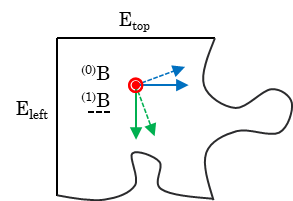
\includegraphics{sections/solver/images/orientation.png}
    \caption{Gewünschte Orientierung des Teils (linke, obere Ecke) durch Optimierung der Orientierung der Basis ${}^{(1)}B$.}
    \label{fig:orientation}
\end{figure}
Hierfür sollte die y-Koordinate des Kantenvektors ${}^{(0)}E_{top}$ der oberen Kante und die x-Koordinate des Kantenvektors  ${}^{(0)}E_{left}$ nach Referenzsystem ${}^{(0)}B$ Null betragen. Hierfür werden die genannten Kannten von ihrer lokalen Basis ${}^{(1)}B$ in das Referenzsystem rotiert, wobei anstatt der Transformationsmatrix ${}^{(0,1)}T$ nur die angenäherte Variante der Rotationsmatrix $R$ (siehe \autoref{approx_rot}) verwendet wird, da hier nur die Orientierung von Bedeutung ist.
\begin{gather}
    {}^{(0)}E_{top} = {}^{(0,1)}R {}^{(1)}E_{top}\\
    {}^{(0)}E_{left} = {}^{(0,1)}R {}^{(1)}E_{left}
\end{gather}
Daraus ergibt sich für die y-Koordinate der oberen Kante ${}^{(0)}E_{top,y}$ bzw. für die x-Koordinate der linken Kante ${}^{(0)}E_{left,x}$
\begin{gather}
    \begin{bmatrix}
        {}^{(0)}E_{top,y}\\
        {}^{(0)}E_{left,x}
    \end{bmatrix} = 
    \begin{bmatrix}
         c_{0,1} {}^{(1)}E_{top,x} - s_{0,1} {}^{(1)}E_{top,y} & 0 & 0\\
         - s_{0,1} {}^{(1)}E_{left,x}  - c_{0,1} {}^{(1)}E_{left,y} & 0& 0
    \end{bmatrix}
    \begin{bmatrix}
        \phi_{1}\\
        x_1\\
        y_1
    \end{bmatrix} +
    \begin{bmatrix}
        s_{0,1} {}^{(1)}E_{top,x} + c_{0,1} {}^{(1)}E_{top,y}\\
        c_{0,1} {}^{(1)}E_{left,x} -s_{0,1} {}^{(1)}E_{left,y}
    \end{bmatrix}
\end{gather}
Diese können nun analog in die Matrix $A$ und den Vektor $b$ mit aufgenommen werden.

\paragraph{Lösung des Least Squares Problems}
Mit dem linearen Zusammenhang $\epsilon^* = A^*x+b^*$ kann das Least Square Problem aus \autoref{gl:leastsquare} neu formuliert werden.
% \begin{gather}
%     \arg\min_x F(x) \text{, mit }\nonumber\\
%     \begin{align}
%         F(x) &= \frac{1}{2} \epsilon^*^T\epsilon^*\nonumber\\
%         &= \frac{1}{2} (A^*x+b^*)^T(A^*x+b^*)\nonumber\\
%         &= \frac{1}{2} x^TA^*^TA^*x + b^*^TA^*x + x^TA^*b^* + b^*^Tb^*
%     \end{align}
% \end{gather}
% Durch Ableiten und Nullsetzen der Ableitung der kovexen Funktion $F(x)$ erhalten wir das globale Minimum. 
% \begin{gather}
%     \frac{d}{dx}F(x) = x^TA^*^TA^* + b^*^TA^* = 0\\
%     x=-(A^*^TA^*)^{-1} A^*^Tb^*
% \end{gather}

Die Inverse der symmetrischen und quadratischen Matrix lässt sich effizient über die Singulärwertzerlegung berechnen (SVD).

Aufgrund der approximation der Rotationsmatrix mit der Kleinwinkelnäherung kann es sein, dass die ermittelte Lösung nicht dem tatsächlichen Optimum entspricht. Allerdings kann durch mehrmaliges Iterieren bei vorheriger Übertragung des Lösungs-Feinjustierwinkels auf den neuen Vorrotationswinkel für Konvergenz zum Optimimum gesorgt werden.


\paragraph{Ergebnisse}
In \autoref{fig:corner_puzzle_img} und \autoref{fig:puzzle_img} sind die Ergebnis der Implementierung des beschriebenen Optimierungsverfahrens dargestellt. \autoref{fig:corner_puzzle_img} zeigt hierbei eine Darstellung der Puzzleteile anhand ihrer ermittelten Eckpunkte. \autoref{fig:puzzle_img} hingegen, zeigt das tatsächliche, anhand der Optimierungsparameter Zusammengesetzte Puzzle. Es ist anzumerken, dass es sich hierbei, um eine Debug Visualisierung handelt, die beim zusammensetzen der Bilder teilweise zum Abschneiden einzelner Teile führt. Allerdings wurde hier keine weitere Zeit investiert, da diese Artefakte in der tatsächlichen Coin-Visualisierung nicht mehr auftreten. Das hier implementierte Verfahren (/home/vscode/workspace/src/solver/algorithm/src/solver/layout\_optimizer.py) erweist sich als sehr Zeit effizient und benötigt für die Lösung (unter Verwendung des gegeben Puzzles) nur 30 Millisekunden (Siehe Evaluierung des Solvers in /home/vscode/workspace/src/solver/algorithm/postprocessing/finding\_optimal\_layout.ipynb).

\begin{figure}[H]
    \begin{minipage}[t]{0.45\textwidth}
        \centering
        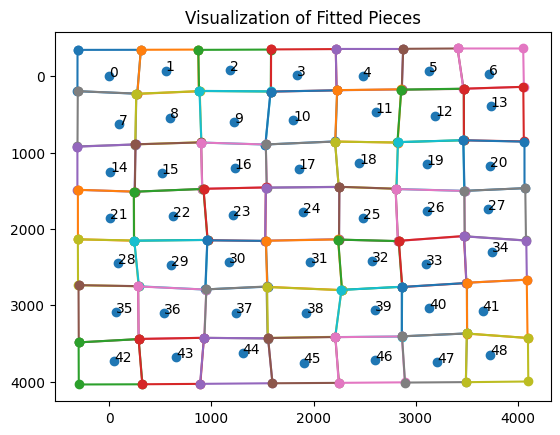
\includegraphics[width=0.95\textwidth]{sections/solver/images/solved_puzzle_edges.png}
        \caption{Eckpunkt-Visualisierung der gelösten Puzzels zur Besseren Darstellung des Optimierungsergebnisses, da hier die angenommenen Eckpunkte dargestellt werden.}
        \label{fig:corner_puzzle_img}
        \end{minipage}
    \hfill
    \begin{minipage}[t]{0.45\textwidth}
        \centering
        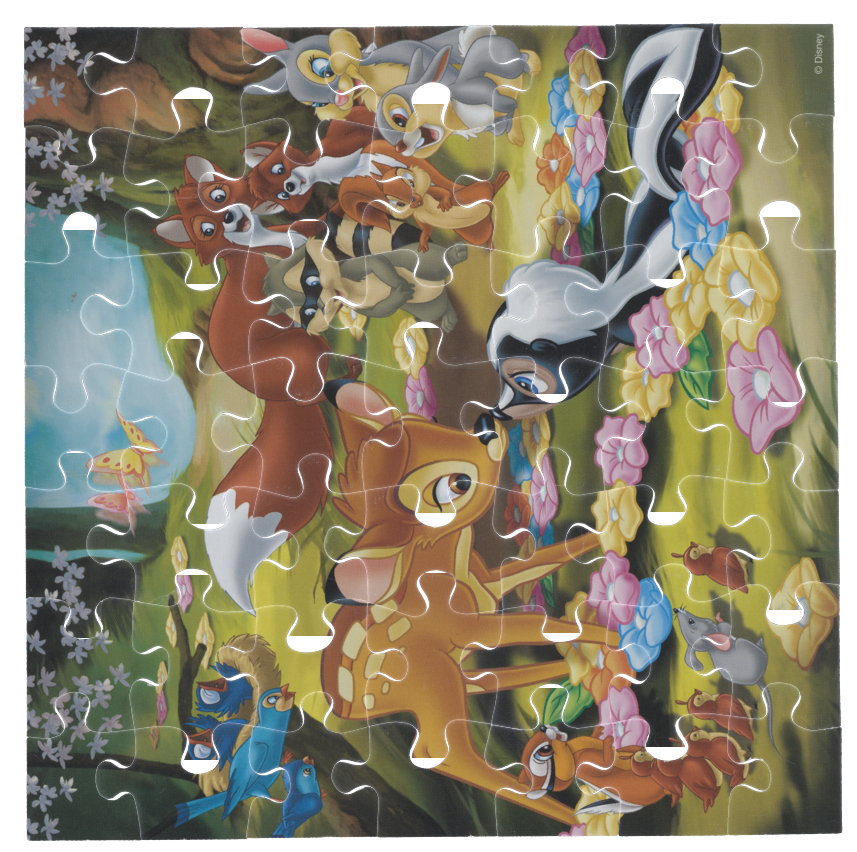
\includegraphics[width=0.7\textwidth]{sections/solver/images/solved_puzzle_img.png}
        \caption{Aus den ermittelten Posen zusammengefügte Puzzle. Teilweise abgeschnittene Puzzleteile sind Artefakte der (Debug-) Visualisierung.}
        \label{fig:puzzle_img}
    \end{minipage}
\end{figure}



\subsubsection[Non Linearer Layout Optimierer]{Non Linearer Layout Optimierer \myAuthor{Mohammadjavad Zamani Pozveh}}
\paragraph{Motivation} Das Ziel des nichtlinearen Optimierers ist es, die Gesamtabstände zwischen benachbarten Ecken von Puzzleteilen zu minimieren, was zu einer optimalen Zusammenstellung führt. Diese Methode berücksichtigt die exakte Drehung jedes Puzzleteils, ohne dabei Rotationsschätzungen zu verwenden. Dies führt zu nichtlinearen Operationen, wie die Drehung von Vektoren oder euklidische Abstände zwischen Ecken, die mit linearen Methoden allein und ohne Schätzungen nicht gelöst werden können. Durch die Anwendung einer Fehlerminimierung stellt der Optimierer schließlich sicher, dass der Gesamtabstand zwischen den entsprechenden Ecken des Puzzles minimiert wird. Mit diesem Ansatz wird ein globales Optimum erreicht. 

\paragraph{Verfahren} Wie bereits erwähnt, ist ein gelöstes Puzzle mit $N$ Zeilen und $M$ Spalten gegeben. Für jedes Puzzleteil sind die Positionen seiner Ecken relativ zum Bildkoordinatensystem angegeben, welches in der oberen linken Ecke des Bildes beginnt (siehe \autoref{fig:piece_corner_cordinate}).


\begin{figure}[H]

    \begin{minipage}[t]{0.45\textwidth}
        \centering
        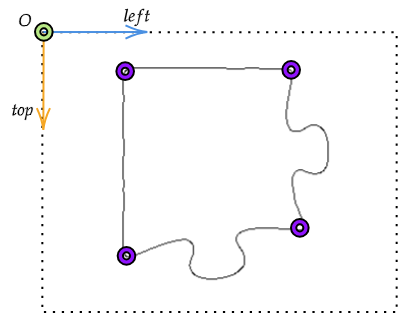
\includegraphics[width=0.95\textwidth]{sections/solver/images/puzzle_image_cordinates.png}
        \caption{Positionen der Ecken im Bildkoordinatensystem (top, left).}
        \label{fig:piece_corner_cordinate}
        \end{minipage}
    \hfill
    \begin{minipage}[t]{0.45\textwidth}
        \centering
        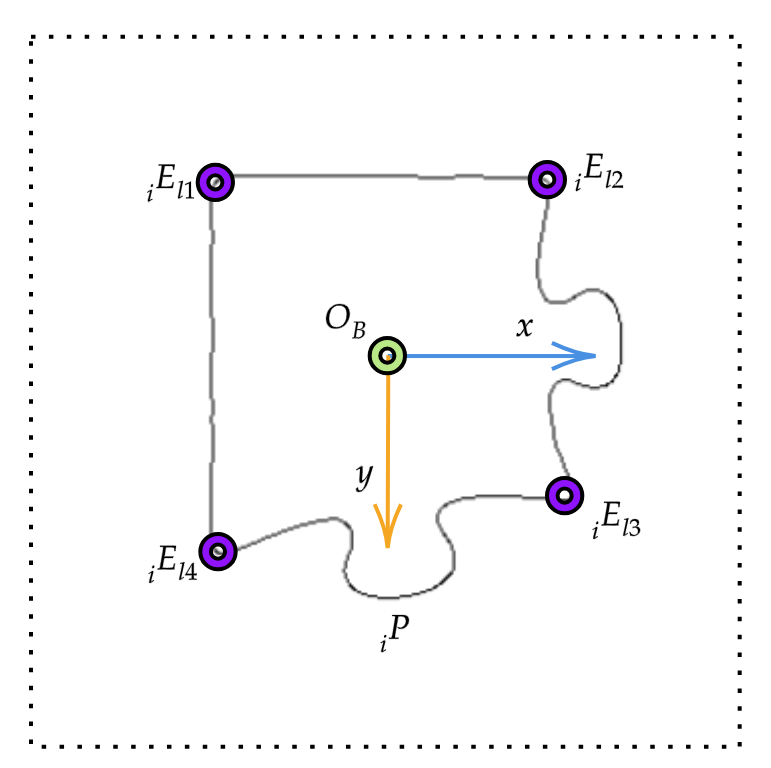
\includegraphics[width=0.7\textwidth]{sections/solver/images/puzzle_image_local_cordinate.png}
        \caption{Positionen der Ecken relativ zum Mittelpunkt des Bildes (padded image).}
        \label{fig:piece_local_cordinate}
    \end{minipage}
\end{figure}

Um die Fehlerfunktion zu definieren, müssen zuerst alle Teile in ein globales Koordinatensystem eingefügt werden und die Position jeder Ecke relativ zu diesem Koordinatensystem berechnet werden. Um die Berechnungen für die Fehlerfunktion zu reduzieren, wird die Position der Ecken jedes Puzzleteils in bekannte und unbekannte Variablen zerlegt, wobei die bekannten Variablen nur einmal berechnet und für weitere Berechnungen verwendet werden.



Zunächst wird jedes Bild so aufgefüllt, dass es ein Quadrat bildet, und der Mittelpunkt des quadratisch aufgefüllten Bildes wird als Ursprung des neuen Koordinatensystems gewählt, im Gegensatz zur oberen linken Ecke. Alle Eckpositionen werden dann in dieses neue Koordinatensystem umgewandelt und gespeichert (siehe \autoref{fig:piece_local_cordinate}):

\begin{equation}
_{i} E_{l1} \ =\ _{i} E_{B1} \ -\ O_{B}
\end{equation}

wobei $\mathbf{{}_{i}E_{1l}}$ die Position der ersten Ecke des Puzzleteils $\mathbf{i}$ relativ zum Mittelpunkt $\mathbf{O_{B}}$ des Bildes ist und $\mathbf{{}_{i}E_{B1}}$ die Position derselben Ecke im Bild-Koordinatensystem ist.


Diese Veränderung des Ursprungs vereinfacht die Berechnungen der neuen Eckpositionen nach der Drehung des Bildes. Anschließend werden die Eckkoordinaten basierend auf ihrer Position (z.B. obere linke oder untere rechte Ecke) sortiert und in einer Matrix der Größe $2N \times 2M$ gespeichert.

Als nächstes werden die Teile im globalen Koordinatensystem positioniert, und die Position des Mittelpunkts des Bildes relativ zum Ursprung des globalen Koordinatensystems wird als globale Teileposition in einer Matrix der Größe $N \times M$ gespeichert (siehe \autoref{fig:pieces_global_system}). Nun kann die Position jeder Ecke im globalen Koordinatensystem wie folgt berechnet werden:

\begin{equation}
_{i} E_{g1} \ =\ _{i} E_{l1} \ +\ _{i} P
\end{equation}


wobei $\mathbf{{}_{i}E_{g1}}$ die Position der ersten Ecke des Puzzleteils $\mathbf{i}$ und $\mathbf{{}_{i}P}$ die Position des ersten Puzzleteils im globalen Koordinatensystem ist.


Es wird angenommen, dass jedes Teil durch einen Vektor $\mathbf{T}$ translatiert und um einen Winkel $\theta$ gedreht wird, um seine Endposition zu erreichen. Daher können die endgültigen Koordinaten der Ecken jedes Puzzleteils basierend auf den bekannten Variablen der Teil-Position und der lokalen Eck-Position sowie den unbekannten Variablen $\mathbf{T}$ und $\theta$ ausgedrückt werden. Nach der Verschiebung und Drehung werden die Eckpositionen im globalen Koordinatensystem wie folgt berechnet:


\begin{equation}
_{i} E\prime_{g1} \ =\ R_{\theta _{i}} \cdot _{i} E_{g1} \ +\ _{i} P +\ _{i} T 
\end{equation}


\begin{equation}
R_{\Theta _{i}} =\begin{bmatrix}
\cos( \theta _{i}) & -\sin( \theta _{i})\\
\sin( \theta _{i}) & \cos( \theta _{i})
\end{bmatrix}\\
\end{equation}


wobei $\mathbf{{}_{i}E\prime_{g1}}$ die Position der ersten Ecke vom Puzzleteil $\mathbf{i}$ nach der Verschiebung und Drehung ist, $\mathbf{{}_{i}T}$ der Translationsvektor des Puzzleteils und $\mathbf{R_{\theta _{i}}}$ die Rotationsmatrix für den Winkel $\mathbf{\theta _{i}}$ ist. 

Die $\mathbf{{}_{i}P}$ und $\mathbf{{}_{i}E_{g1}}$ müssen nur einmal berechnet werden und bleiben bei jeder Auswertung der Fehlerfunktion und folglich der Eckposition unverändert.

\begin{figure}[H]
    \centering
    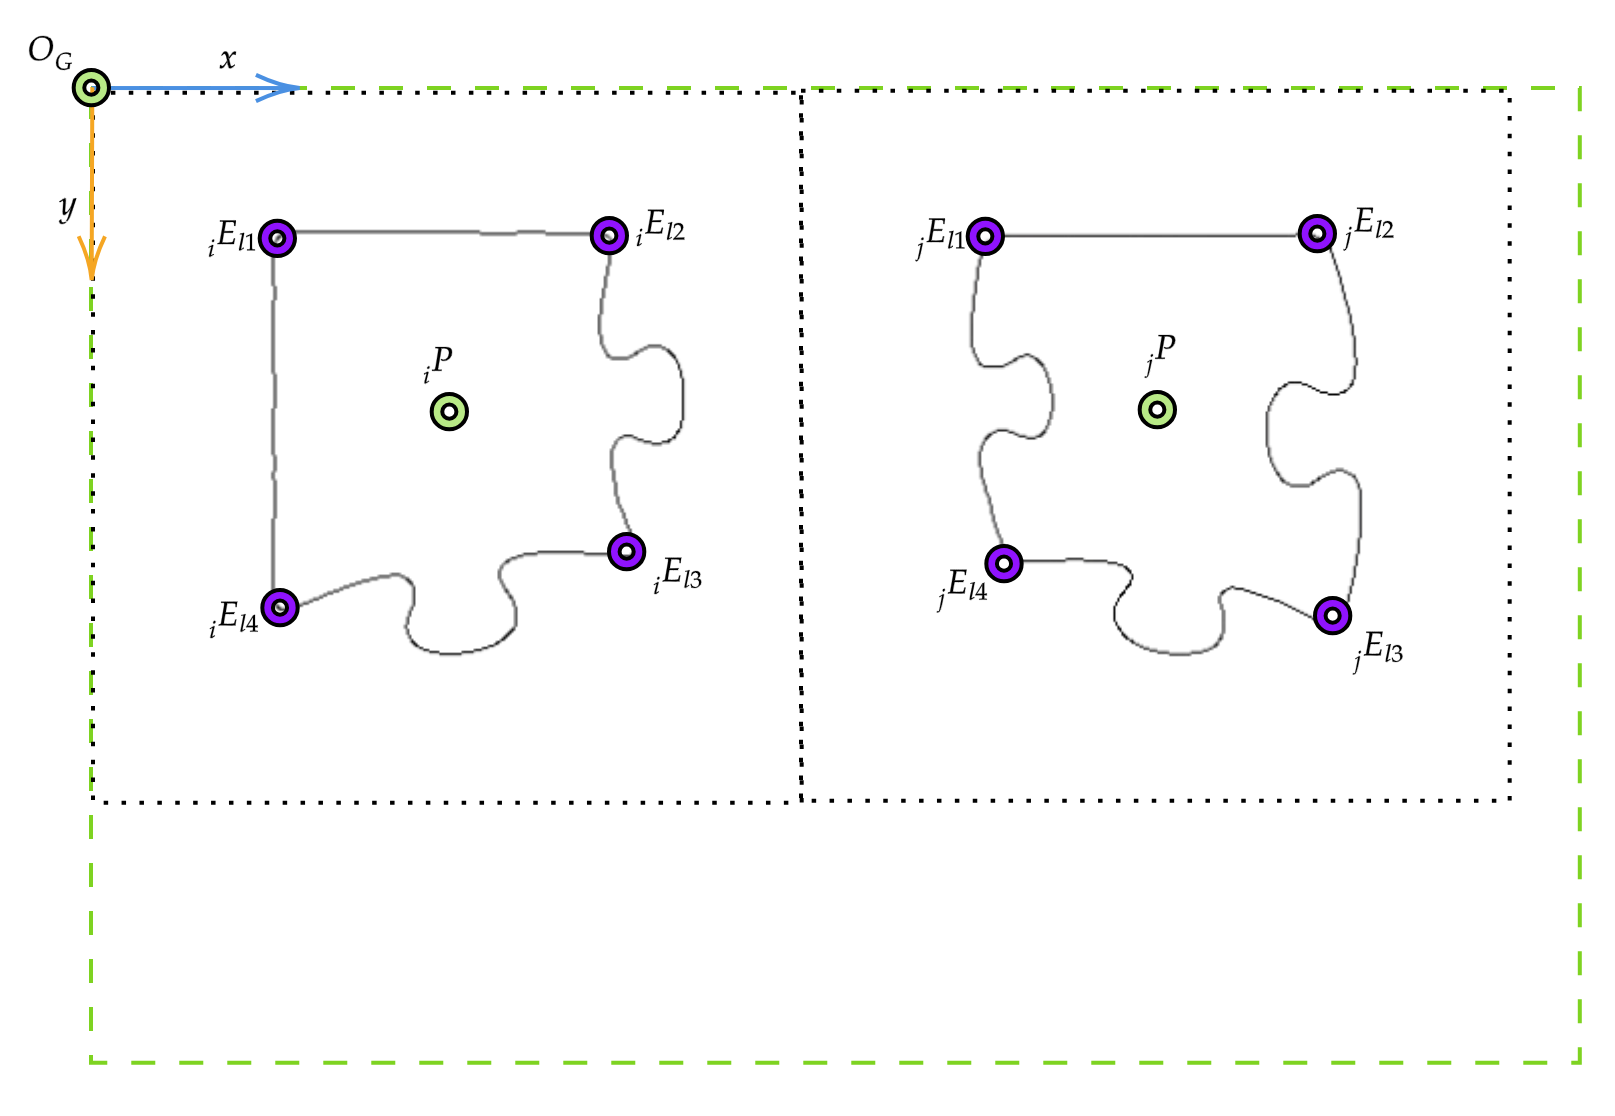
\includegraphics[width=0.95\textwidth]{sections/solver/images/pieces_global_system.png}
    \caption{Positionierung der Puzzleteile im globalen Koordinatensystem. Wobei $\mathbf{{}_{i}P}$ und $\mathbf{{}_{j}P}$ die Positionen von Puzzleteilen $\mathbf{{i}}$ und $\mathbf{{j}}$ im globalen Koordinatensystem sind.}
    \label{fig:pieces_global_system}
\end{figure}

\begin{figure}[H]
    \centering
    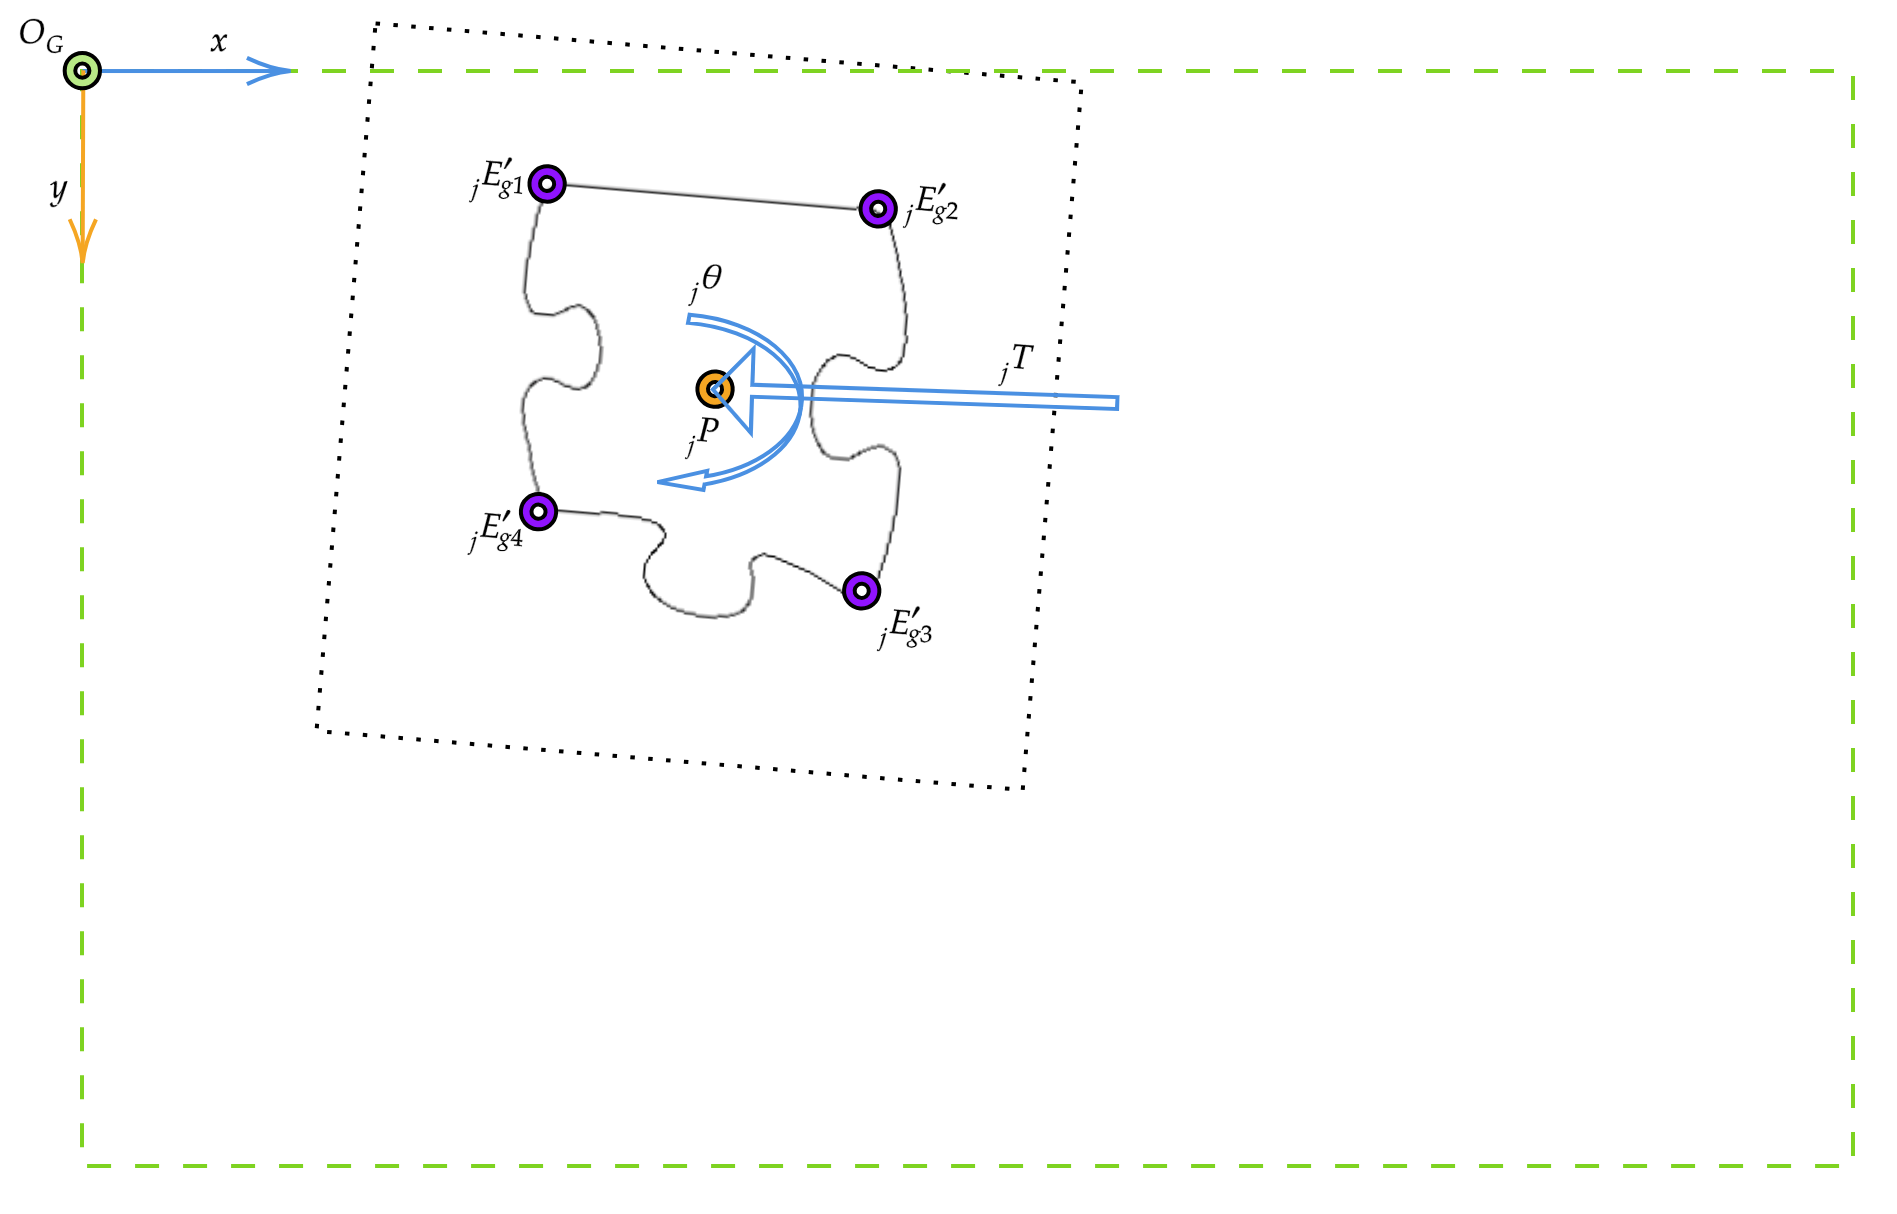
\includegraphics[width=0.95\textwidth]{sections/solver/images/piece_rotation_translation.png}
    \caption{Position der Ecken nach Durchführung von Translation $\mathbf{T}$ und Drehung $\mathbf{\theta}$.}
    \label{fig:pieces_translation_rotation}
\end{figure}

Mit den Eckpositionen im globalen Koordinatensystem kann die Fehlerfunktion als Summe aller euklidischen Distanzen zwischen benachbarten Ecken definiert werden (siehe \autoref{fig:corner_distance}). Dies wird mathematisch dargestellt als:

\begin{equation}
F_{\text{err}}(\overline{E_{g}}) = \sum_{\text{Nachbarn Ecken $\mathbf{i,j}$}} \| \mathbf{E}_{gi} - \mathbf{E}_{gj} \|^2
\end{equation}

wobei $\mathbf{E}_{gi}$ und $\mathbf{E}_{gj}$ die Positionen benachbarter Ecken sind und $\mathbf{\overline{E_{g}}}$ die Positionsmatrix aller Ecken ist.

\begin{figure}[H]
    \centering
    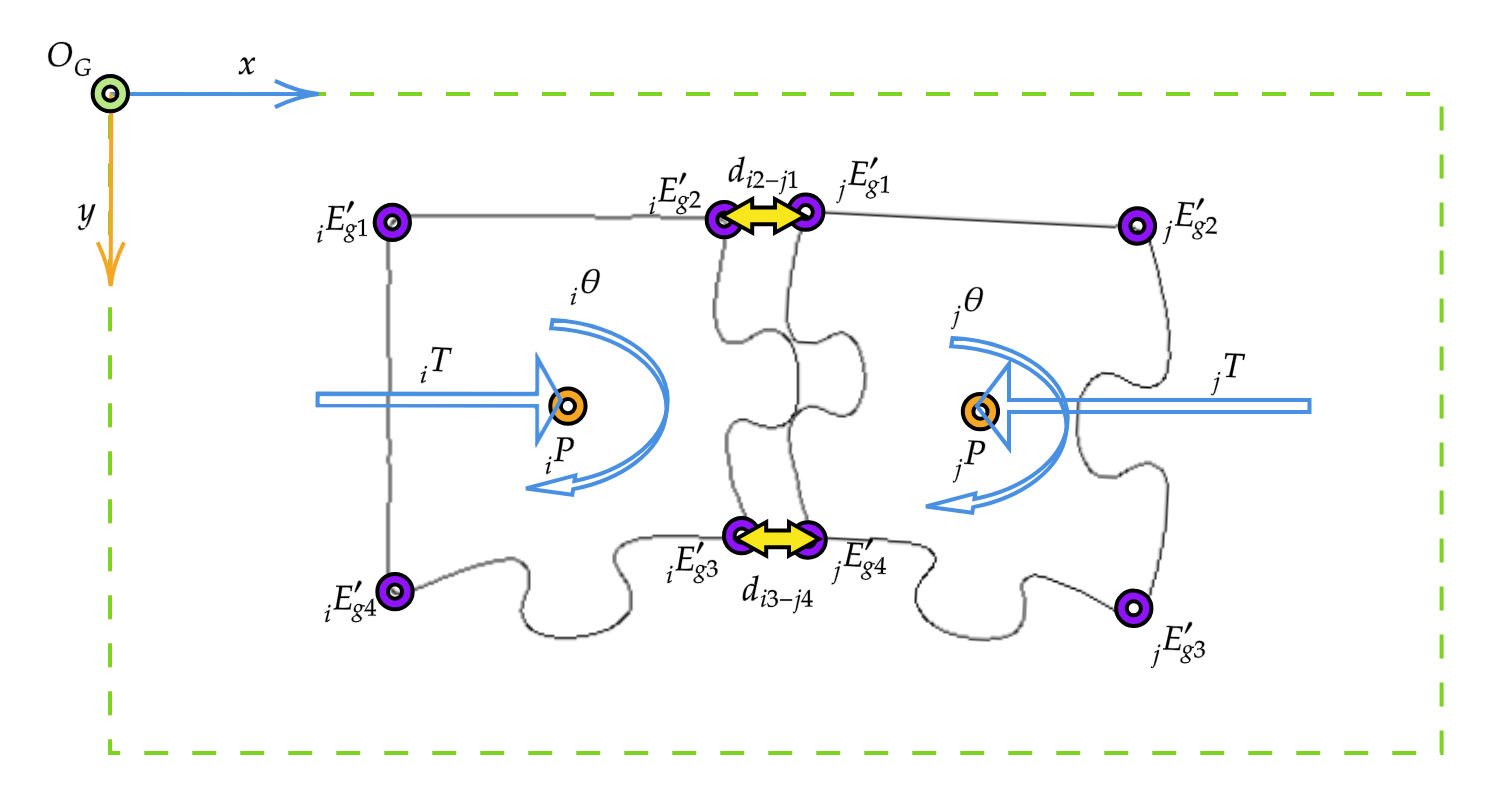
\includegraphics[width=0.95\textwidth]{sections/solver/images/corner_distance.png}
    \caption{Distanzen zwischen benachbarten Ecken ($\mathbf{d_{i2-j1}}$} und $\mathbf{d_{i3-j4}}$) nach Durchführung von Translation $\mathbf{T}$ und Drehung $\mathbf{\theta}$.
    \label{fig:corner_distance}
\end{figure}

\paragraph{Minimierung der Fehlerfunktion}
Mit der definierten Fehlerfunktion ist der nächste Schritt, diese mithilfe von \texttt{scipy.minimize} zu minimieren. Es ist erforderlich, einen Vektor der Unbekannten zu erstellen und eine Anfangsschätzung für jede von ihnen bereitzustellen. Der Vektor der Unbekannten ist wie folgt definiert:

\begin{equation}
X\ =\ \begin{bmatrix}
_{i} T_{x} & _{i} T_{y} & _{i} \theta 
\end{bmatrix}_{1\times 3MN}
\end{equation}

wobei $\mathbf{X}$ der Vektor der Unbekannten ist. Da für jedes Puzzleteil 3 Unbekannte existieren, hat der Vektor eine Größe von $\mathbf{1\times 3MN}$. $\mathbf{_{i} T_{x}}$ und $\mathbf{_{i} T_{y}}$ sind Translationen in Richtung der $\mathbf{x}$- und $\mathbf{y}$-Achsen. $\mathbf{_{i} \theta}$ ist der Drehwinkel. Alle Werte beziehen sich auf Puzzleteil $\mathbf{i}$.


Die Anfangsschätzung ist besonders wichtig, insbesondere wenn die zu optimierende Funktion nicht kontinuierlich ist. Wie im folgenden Abschnitt besprochen (\ref{sec_combination_linear_non_linear}), kann die Anfangsschätzung das Ergebnis eines vorherigen linearen Optimierers sein, auf dem dann weitere nichtlineare Optimierungen durchgeführt werden können.

Für jede unbekannte Variable sollten obere und untere Grenzen definiert werden. Diese Begrenzung stellt sicher, dass der Optimierer effizient arbeitet, indem er unnötige Bewegungen einschränkt und sich auf die Bereiche konzentriert, die für die Minimierung des Fehlers am relevantesten sind. Eine gut definierte Begrenzung kann die Anzahl der erforderlichen Iterationen reduzieren und somit die Gesamtzeit für die Optimierung verkürzen. 

Die Berechnung der Grenzen hängt wesentlich vom Abstand der Ecke jedes  Puzzleteils zu seinem Rand ab. In unserem Programm sind die Grenzen jedes Puzzleteils auf die Hälfte der Gesamtgröße des Puzzles festgelegt. Diese Konfiguration der Grenzen ist so gestaltet, dass alle Puzzleteile sich in Richtung der oberen linken Seite des globalen Koordinatensystems bewegen können, indem den negativen Werten der unbekannten Variablen mehr Spielraum gegeben wird als den positiven. 

In der Praxis bedeutet dies, dass für jede unbekannte Variable $T_x$, $T_y$ (Translationen) und $\theta$ (Rotation) folgende Grenzen definiert werden:
\begin{itemize}
    \item $T_x \in [-\frac{1}{2} \text{Puzzlegröße-x}, \frac{1}{10} \text{Puzzlegröße-x}]$
    \item $T_y \in [-\frac{1}{2} \text{Puzzlegröße-y}, \frac{1}{10} \text{Puzzlegröße-y}]$
    \item $\theta \in [-\frac{\pi}{4}, \frac{\pi}{4}]$
\end{itemize}

Diese asymmetrischen Grenzen ermöglichen eine größere Flexibilität in den negativen Richtungen, was die Bewegung der Puzzleteile in Richtung des Ursprungs fördert.

Es ist wichtig zu beachten, dass der Bereich der unbekannten Drehung $\theta$ sich von den Translationen unterscheidet, daher muss $\theta$ zuerst auf die gleiche Dimension wie die Translationen normiert werden. Diese Normierung stellt sicher, dass der Optimierer alle Unbekannten konsistent behandelt.

Als Nächstes wird die Fehlerfunktion zusammen mit dem Vektor der Grenzen und dem Vektor der ersten Anfangsschätzung an den Optimierer übergeben, um das Minimum der Fehlerfunktion zu erhalten.

\paragraph{Optimierungsmethode und Konfiguration}
Die gewählte Optimierungsmethode für dieses Problem ist L-BFGS-B (Limited-memory Broyden-Fletcher-Goldfarb-Shanno with Box constraints). Diese Methode ist besonders geeignet für Probleme mit großen Datenmengen und nichtlinearen Funktionen, wie es bei der Anordnung von Puzzleteilen der Fall ist. L-BFGS-B ist eine Erweiterung des BFGS-Algorithmus, die speziell für große Optimierungsprobleme entwickelt wurde. Der Algorithmus verwendet eine begrenzte Menge an Speicher (daher "limited-memory"), was ihn besonders effizient für Probleme mit vielen Variablen macht. Weitere Vorteile sind:

\begin{itemize}
    \item \textbf{Speichereffizienz:} Durch die Verwendung von begrenztem Speicher ist L-BFGS-B effizienter als andere Optimierungsalgorithmen, die den gesamten Hessian (die zweite Ableitungsmatrix) speichern und manipulieren müssen.
    \item \textbf{Handhabung von Box-Beschränkungen:} L-BFGS-B kann direkt mit Box-Beschränkungen umgehen, d.h. es können einfache obere und untere Grenzen für die Variablen festgelegt werden, was für unser Problem der Puzzleanordnung ideal ist.
    \item \textbf{Skalierbarkeit:} Die Methode skaliert gut mit der Anzahl der Variablen und ist daher für große Optimierungsprobleme geeignet (für ein Puzzle mit $\mathbf{x}$ Teilen haben wir $\mathbf{3 \cdot x}$ unbekannte Variablen).
\end{itemize}

Für eine optimale Leistung der L-BFGS-B Methode müssen einige Konfigurationsparameter geeignet gewählt werden:

\begin{itemize}
    \item \textbf{Startwerte (Anfangsschätzung):} Die Wahl guter Startwerte ist entscheidend. In unserem Fall können die Startwerte die Positionen und Drehungen der Puzzleteile aus einer vorherigen linearen Optimierung sein oder ganz zufällig ausgewählt werden.
    \item \textbf{Schrittweite:} Die Schrittweite, oder \texttt{stepsize}, ist ein wichtiger Parameter, der die Größe der Schritte beeinflusst, die der Optimierer bei der Suche nach dem Minimum unternimmt. Eine zu große Schrittweite kann dazu führen, dass der Optimierer über das Minimum hinaus schießt, während eine zu kleine Schrittweite die Konvergenz verlangsamen kann.
    \item \textbf{Grenzen:} Die oben definierten Grenzen für die Variablen $T_x$, $T_y$ und $\theta$ helfen, die Suchregion des Optimierers einzugrenzen und die Konvergenz zu beschleunigen.
    \item \textbf{Toleranzen:} Die Parameter für Toleranzen, wie \texttt{gtol} (Gradienten-Toleranz) und \texttt{ftol} (Funktions-Toleranz), beeinflussen, wann der Optimierer die Suche stoppt. Diese sollten so gewählt werden, dass sie eine gute Balance zwischen Präzision und Rechenzeit bieten (Wenn die Puzzleteile voneinander entfernt sind, können wir mit einer großen Zahl beginnen, z. B. 10, und wenn sie sich einander nähern, können wir sie auf 0,1 reduzieren).
    \item \textbf{Maximale Iterationen:} Die maximale Anzahl an Iterationen, \texttt{maxiter}, sollte ausreichend groß gewählt werden, um die Konvergenz zu ermöglichen, aber nicht so groß, dass unnötig Rechenzeit verbraucht wird. Ein typischer Wert könnte bei 100-1000 Iterationen liegen.
\end{itemize}

Trotz ihrer vielen Vorteile hat die L-BFGS-B Methode auch einige Einschränkungen:

\begin{itemize}
    \item \textbf{Lokales Optimum:} L-BFGS-B kann in lokale Optima geraten, insbesondere wenn die Startwerte weit von einem globalen Optimum entfernt sind. Daher ist die Wahl guter Startwerte entscheidend.
    \item \textbf{Nicht geeignet für diskrete Variablen:} L-BFGS-B ist für kontinuierliche Variablen konzipiert und nicht für Probleme mit diskreten Variablen geeignet. Zum Beispiel, wenn die Eckpositionen nicht korrekt erkannt werden oder andere Faktoren dazu beitragen, dass die Fehlerfunktion diskret ist, würde diese Methode keine optimale Ausgabe liefern.
    \item \textbf{Sensitivität gegenüber Parametereinstellungen:} Die Methode kann empfindlich auf die Einstellungen der Konfigurationsparameter reagieren. Falsche Einstellungen können die Konvergenz verlangsamen oder sogar verhindern.
\end{itemize}

Es kann vorkommen, dass die optimierten Werte in einem lokalen Minimum enden (siehe \autoref{fig:nonoptim_local_minima}). In einem solchen Fall gibt es zwei mögliche Ansätze, um dieses Problem zu lösen:



\textbf{Zufälliges Rauschen hinzufügen}: Der erste Ansatz besteht darin, dem Ergebnis des Optimierers ein kleines zufälliges Rauschen hinzuzufügen und die optimierten Werte erneut in den Optimierer einzugeben. Dieses zufällige Rauschen kann dem Optimierer helfen, aus dem lokalen Minimum herauszukommen, indem es ihn dazu bringt, neue Bereiche des Lösungsraums zu erkunden. Der Nachteil dieser Methode ist jedoch, dass sie iterativ durchgeführt werden muss, um sicherzustellen, dass der Optimierer tatsächlich das globale Optimum gefunden hat. Diese Iterationen können zeitaufwendig sein.


\textbf{Kombination von linearer und nichtlinearer Optimierung}: Der zweite Ansatz ist im \autoref{sec_combination_linear_non_linear} diskutiert.


\begin{figure}[H]
    \centering
    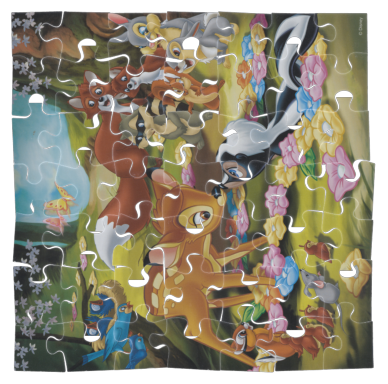
\includegraphics[width=0.45\textwidth]{sections/solver/images/noptim_local_minima.png}
    \caption{Optimuzer ist in einem lokalen Minima gelandet. ($\mathbf{F_{\text{err}} = 3.75e+3}$)}
    \label{fig:nonoptim_local_minima}
\end{figure}

\paragraph{Ergebnisse}
In \autoref{fig:nonoptim_start_puzzle} ist das Puzzle zu sehen, mit dem der Optimierer gestartet ist, und in Abbildung \autoref{fig:nonoptim_end_result} das Ergebnis. Der Wert der Fehlerfunktion liegt zu Beginn der Optimierung bei $\mathbf{F_{\text{err}} = 1.23e+5}$ und wird nach der Optimierung auf den Wert von $\mathbf{F_{\text{err}} = 6.62e+2}$ reduziert. Die Laufzeit des Optimierers hängt von den Startwerten, Konfiguration und auch von der Hardware ab, auf der er läuft. Auf meinem System dauerte jeder Durchlauf durchschnittlich über 90  Sekungden (mit dem gegebenen Puzzle), was relativ lang ist, aber es kann durch die Wahl besserer Startwerten verbessert werden (Siehe Ablauf des Optimierers in src/solver/algorithm/postprocessing/non-linear-optimal-layout.ipynb).

\begin{figure}[H]
    \begin{minipage}[t]{0.45\textwidth}
        \centering
        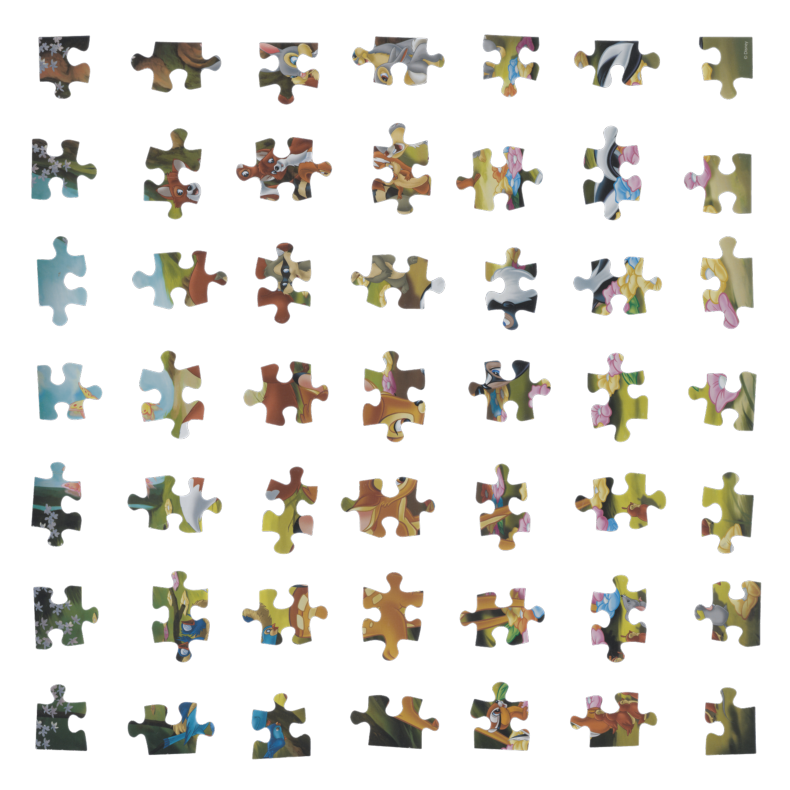
\includegraphics[width=0.95\textwidth]{sections/solver/images/noptim_start_puzzle.png}
        \caption{Layout des Puzzles vor der Optimierung ($\mathbf{F_{\text{err}} = 1.23e+5}$)}
        \label{fig:nonoptim_start_puzzle}
        \end{minipage}
    \hfill
    \begin{minipage}[t]{0.45\textwidth}
        \centering
        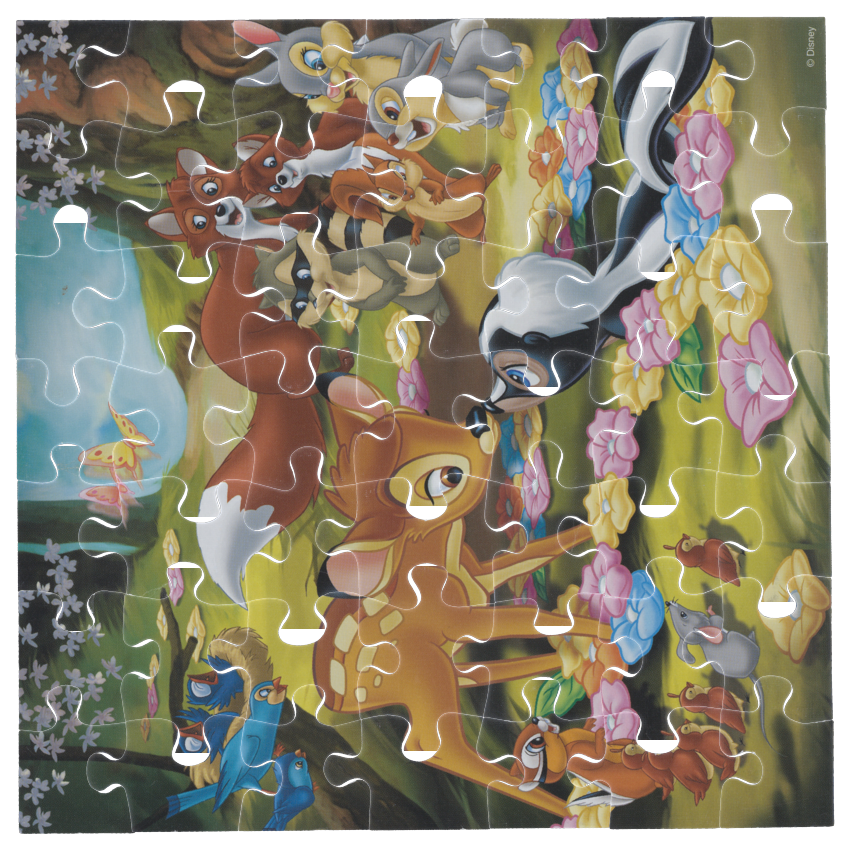
\includegraphics[width=0.95\textwidth]{sections/solver/images/noptim_solved.png}
        \caption{Layout des Puzzles nach der Optimierung ($\mathbf{F_{\text{err}} = 6.62e+2}$)}
        \label{fig:nonoptim_end_result}
    \end{minipage}
\end{figure}


\paragraph{Fazit}
Die Fehlerfunktion wird durch die euklidischen Distanzen zwischen den benachbarten Ecken definiert. Der Optimier minimiert die Gesamtabstände zwischen benachbarten Ecken der Puzzleteile, indem er sowohl Translationen als auch Rotationen berücksichtigt. Die Auswahl geeigneter Startwerte, die Definition von Grenzen für die Variablen und die korrekte Konfiguration der Optimierungsparameter spielen eine entscheidende Rolle für die Effizienz und Genauigkeit der Methode. Wenn der Optimier in einem lokalen Minima bleibt, können Methoden wie das Hinzufügen von zufälligem Rauschen oder die Kombination von linearen und nichtlinearen Optimierungen angewendet werden.


\subsubsection{Kombination von lineareren und nichtlineareren Layout Optimierer [Zamani Pozveh]}
\label{sec_combination_linear_non_linear}
\paragraph{Motivation} Lineare Optimierer sind in der Regel schneller und weniger rechenintensiv als nichtlineare Optimierer. Sie können schnell eine gute erste Annäherung an die optimale Lösung finden, indem sie die Variablen innerhalb eines linearen Modells optimieren. 

Nichtlineare Optimierer können komplexe und nichtlineare Beziehungen besser modellieren. Allerdings kann es passieren, dass sie in lokalen Minima stecken bleiben, insbesondere wenn die Ausgangswerte weit vom globalen Optimum entfernt sind. Durch die Kombination beider Methoden werden die Geschwindigkeit und Effizienz der linearen Optimierung mit der Genauigkeit der nichtlinearen Optimierung vereint.

Im Kontext der Anordnung von Puzzleteilen kann der lineare Optimierer schnell eine grobe Anordnung basierend auf den Ecken der Puzzleteile finden. Der nichtlineare Optimierer verfeinert dann die Positionen und Rotationen, um die minimale Gesamtdistanz zwischen den benachbarten Ecken zu erreichen. Diese zweistufige Optimierungsmethode stellt sicher, dass die Lösung sowohl effizient als auch präzise ist.

\paragraph{Verfahren} Die Ergebnisse der linearen Optimierung werden als Startwerte für den nichtlinearen Optimierer verwendet. Die Grenzen und Startwerte werden so konfiguriert, dass der nichtlineare Optimierer innerhalb der durch den linearen Optimierer definierten Suchregion arbeitet. 

\paragraph{Ergebnisse}
In \autoref{fig:result_of_linear_optimizer} ist die Puzzle-Ausgabe des linearen Optimierers zu sehen, die als Startwerte für den nichtlinearen Optimierer gegeben sind. In Abbildung \autoref{fig:fine_tuned_puzzle} ist das verfeinerte Puzzle zu sehen. Der Wert der Fehlerfunktion wurde von $\mathbf{F_{\text{err}} = 6.81+e2}$ auf $\mathbf{F_{\text{err}} = 6.61e+2}$ reduziert. Der nichtlineare Optimierer hat die Drehung und Position einiger Puzzleteile verbessert(Siehe \autoref{fig:fine_tune_diff}).


Die Laufzeit des Optimierers hängt von den Startwerten, Konfiguration und auch von der Hardware ab, auf der er läuft. Auf meinem System dauerte jeder Durchlauf durchschnittlich unter 15 Sekungden (mit dem gegebenen Puzzle und Ausgabe des linearen Optimierers als Startwerte für den nichtlinearen Optimierer), was akzeptabel ist. Der kann auch durch eine Verbesserung der Konfiguration (nämlich \texttt{stepsize}) reduziert werden (Siehe Ablauf des Verfeinerung in src/solver/algorithm/postprocessing/fine-tunning.ipynb).


\begin{figure}[H]
    \begin{minipage}[t]{0.45\textwidth}
        \centering
        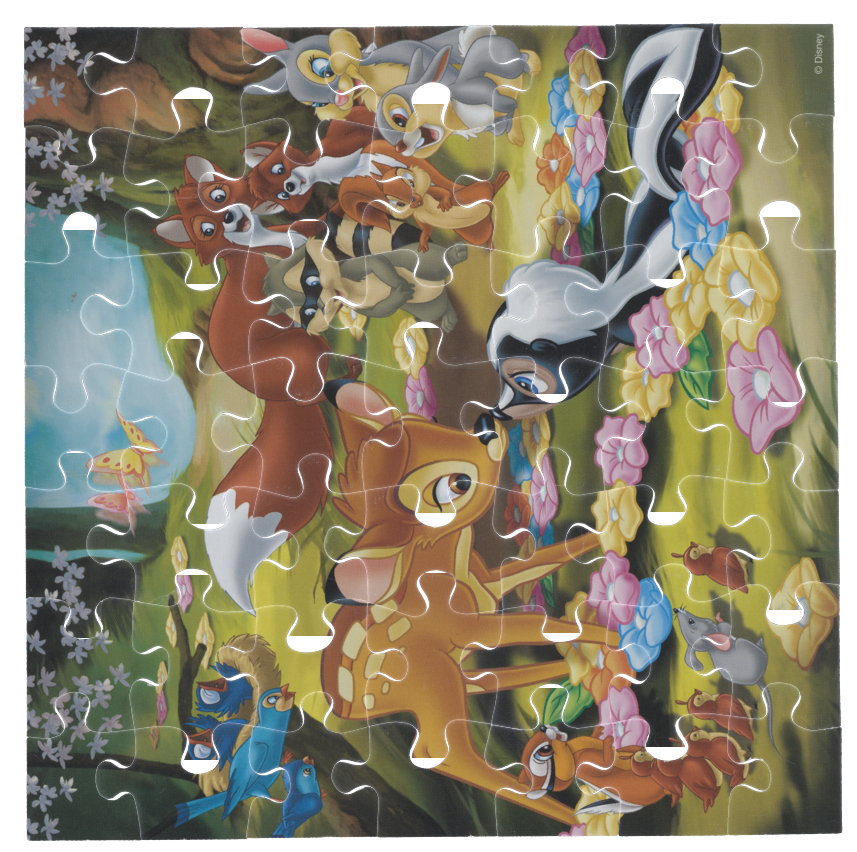
\includegraphics[width=0.95\textwidth]{sections/solver/images/solved_puzzle_img.png}
        \caption{Layout des Puzzles nach linearer Optimierung ($\mathbf{F_{\text{err}} = 6.81+e2}$)}
        \label{fig:result_of_linear_optimizer}
    \end{minipage}
    \hfill
    \begin{minipage}[t]{0.45\textwidth}
        \centering
        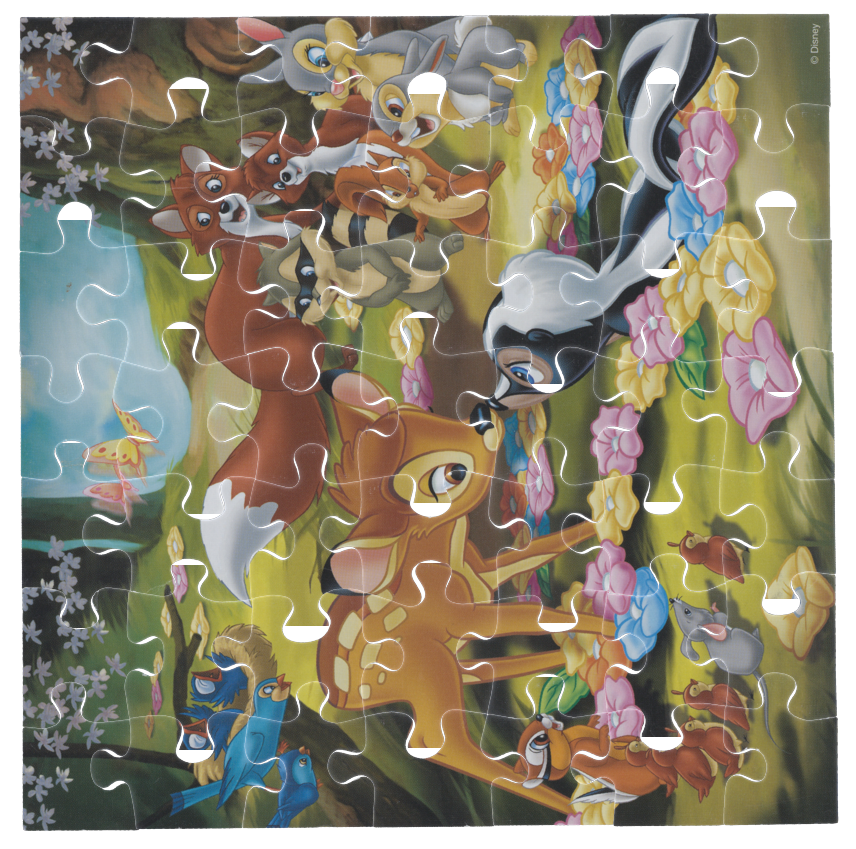
\includegraphics[width=0.95\textwidth]{sections/solver/images/fine_tuned_puzzle.png}
        \caption{Layout des linear optimierten Puzzles nach der Verfeinerung mit dem nichtlinearen Optimierer
        ($\mathbf{F_{\text{err}} = 6.62+e2 }$)}
        \label{fig:fine_tuned_puzzle}
        \end{minipage}
\end{figure}

\begin{figure}[H]
        \centering
        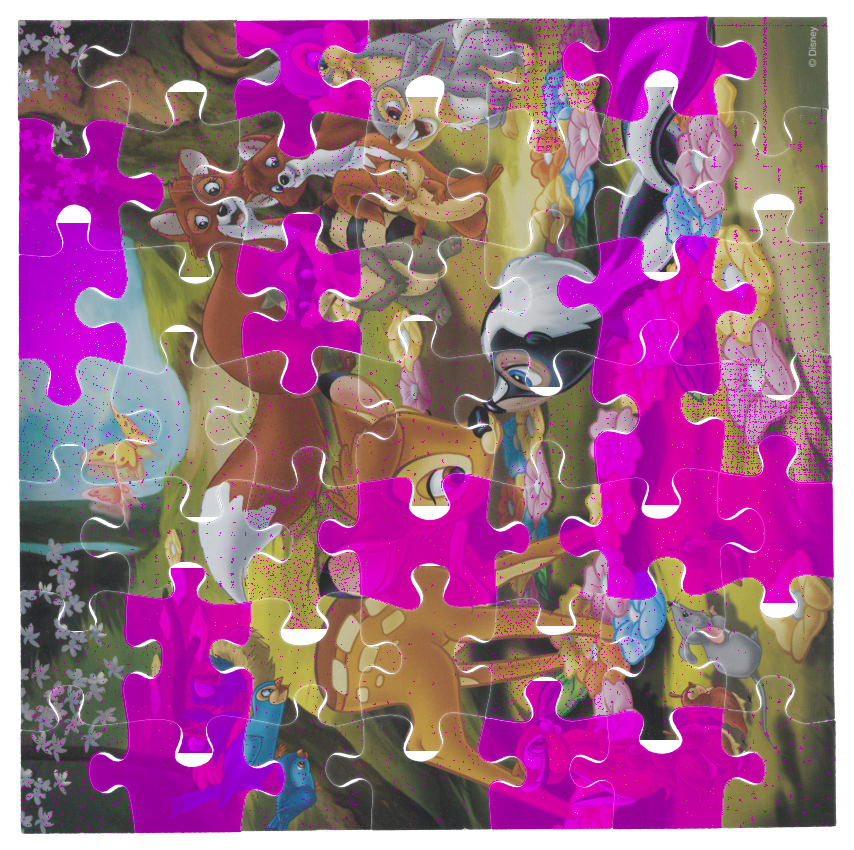
\includegraphics[width=0.95\textwidth]{sections/solver/images/fine_tune_diff.png}
        \caption{Bildunterschied zwischen dem Layout des Puzzles vor und nach der Verfeinerung. Die Puzzleteile, die während des Prozesses verändert wurden, sind rosa gefärbt.}
        \label{fig:fine_tune_diff}
\end{figure}


\paragraph{Fazit} Durch Nutzung eines linearen Optimierers, um eine initiale Annäherung an die optimale Lösung zu finden, wird die Wahrscheinlichkeit reduziert, dass der nichtlineare Optimierer in einem lokalen Minimum stecken bleibt. Diese anfängliche Schätzung liegt näher am globalen Optimum, was dem nichtlinearen Optimierer ermöglicht, schneller und effizienter zu konvergieren. Insgesamt führt diese zweistufige Methode zu einer schneller(als nichtlinearen Optimierer alleine) und präziseren Lösung, da die Vorteile beider Optimierungsansätze kombiniert werden.